\documentclass{article}
\usepackage[top=1.1in, bottom=1.5in, left=1in, right=1in]{geometry}
\usepackage{graphicx}
\usepackage[english,danish]{babel}
\usepackage{enumitem}
\usepackage{pdfpages}
\usepackage{tabu}
\usepackage[normalem]{ulem}
\usepackage[utf8]{inputenc}
\usepackage[T1]{fontenc}

\begin{document}
\title{System Design Document (SDD) for LuckyCalendar}
\author{Mads Frederik Madsen - mfrm, Holger Stadel Borum - hstb and Paw H\o vsgaard Laursen - pawh}
\maketitle
\tableofcontents
\newpage
Version system:\\
First decimal increments whenever we have made complete changes. \\
Second decimal increments for every major change (Not addition).   \\
Third decimal increments for every minor change or major addition.\\

{\tabulinesep=1.2mm
\begin{tabu}{ | p{1.4cm} | p{1.2cm} | p{1.3cm} | p{2.2cm} | p{7cm} |}
    \hline
    Date 		&	Version	& 	Initials			&	Title				&	Description    \\ \hline
    02/10/14	& 	0.1.0	&	pawh, mfrm, hstb	&	Assignment	39		&	Sections 1, 3.1 and 3.2\\ \hline
    06/10/14	& 	0.1.1	&	pawh				&	notes				&	Notes for assignment 40\\ \hline
    09/10/14	& 	0.1.2	&	pawh, mfrm, hstb	&	Assignment	40		&	Added remaining sections in chapter 3\\ \hline
    22/10/14	&	0.1.2.1 & 	pawh, hstb, mfrm	&	Assignment  41		&	Added E/R-diagram of database \\ \hline
    
\end{tabu}
\newpage

\section{Introduction}
	\subsection{Purpose of the system}
		The purpose of our calendar system is to replace the old fashioned paper calendar with a twist. The calendars client will work on most systems and very basic hardware, and as such it may seem quite simplistic. It will implement basic calendar functionality such as keeping track of your appointments, and invite other users to your appointments etc. 

		However, the calendar stands out in its ability to set up appointments between strangers. This functionality, leaves room for extra unknown participants to be added to an event or appointment by our server. These unknown participants will, in their own calendar, make en "empty" appointment, where they want to be invited to a random event near them. That way people lacking, for instance participants for a street party, a bingo tournament or even a 4th player in a tennis double match, will be able to find their extra people. And people lacking something to do while on a business trip to a foreign city, or simply someone who is bored on a Saturday, will get an invitation to try something new, with new and exiting people.

		We call it - LuckyAppointments.

\subsection{Scope of the system}

\subsection{Objectives and success citeria the project}

\subsection{Definitions, acronyms and abbreveations}

\subsection{References}


Version system:\\
First decimal increments whenever we have made complete changes. \\
Second decimal increments for every major change (Not addition).   \\
Third decimal increments for every minor change or major addition.\\

{\tabulinesep=1.2mm
\begin{tabu}{ | p{1.4cm} | p{1.2cm} | p{1.3cm} | p{2.2cm} | p{7cm} |}
    \hline
    Date 		&	Version	& 	Initials			&	Title				&	Description    \\ \hline
    18/09/14	& 	0.1.0	&	pawh mrfm hstb	&	Assignment	37		&	Elementary design, use cases and generic calendar functionality.\\ \hline
    20/09/14	& 	0.2.0	&	pawh mrfm hstb	&	LuckyCalender		&	We have made some major changes to the overall idea of the calendar by adding the idea of LuckyAppointments to the calendar. We have begun on the object analysis of the system.\\ \hline
    21/09/14	& 	0.2.1	&	hstb			&	Sequence Diagram 	&	Added a sequence diagram and renamed the system to LuckyCalendar, so we know the difference between our system and the calendar.\\ \hline
\end{tabu}
}\\\\
VersionControl for minor changes and additions:
https://github.com/Madsen90/BDSA/commits/master
\subsection{Overview}
	\newpage

\section{Current System architecture}
	\section{Current system}
	\newpage

\section{Proposed system architecture}
	\section{Proposed system}
	\subsection{Overview}
	\subsection{Functional Requirements}
	\subsection{Nonfunctional Requirements}				%3_03
		\subsubsection*{}
		{\tabulinesep=1.2mm
\begin{tabu}{ | p{3cm} | p{13cm} |}
    \hline
    Category	 			& 		Requirements \\\hline
    Usability:	  			& 		98\% of the 15-30-year-olds users should be able create, delete, edit appointments and account without prior knowledge, reading or education. \\\hline
    Reliability: 			& 		- Crashes/loss of connection must not cause loss of neither account- or appointment information, none-submitted data may be lost. \\
							&		- It should always be possible to access the server, when the client has Internet connection.\\
							&		- Crashes should be rare - less than 1\% of operations made by a user may lead to a crash. \\ \hline
	Performance:			&		- The system should be scalable - there should only be a hardware limit to the number of appointments or accounts in the system.\\
							&		- The calendar should load fast - there should be a maximum 1-2 second delay on normal computers with 1 mbit connection.\\
							&		- Client should be able to run on a single core 500 MHz CPU.\\ \hline
    Supportability: 		& 		- The system should be documented.  \\
    						&		- Update-able to new browsers and OS'. \\ \hline
	Implementation: 		&		- Requires an Internet connection.\\\hline
	Operation:				&	 	- None. \\\hline
	Legal:					&		- User should agree to terms of use.\\\hline
\end{tabu}
}
\\
	\subsection{System models}							%3_04
		\subsubsection{Scenarios}
			\paragraph{Scenario 1: Create Appointment:}
			 -\\
				\makebox{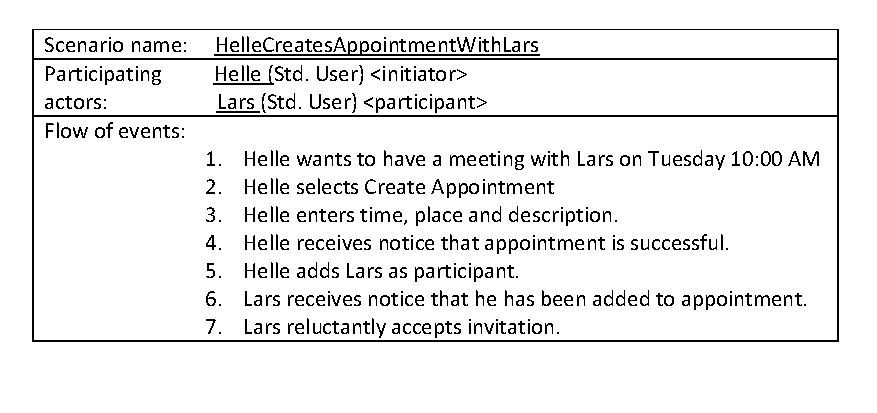
\includegraphics[scale=0.8]{docs/ScCreateApt.pdf}}

			\paragraph{Scenario 2: Create User:}
			 -\\
				\makebox{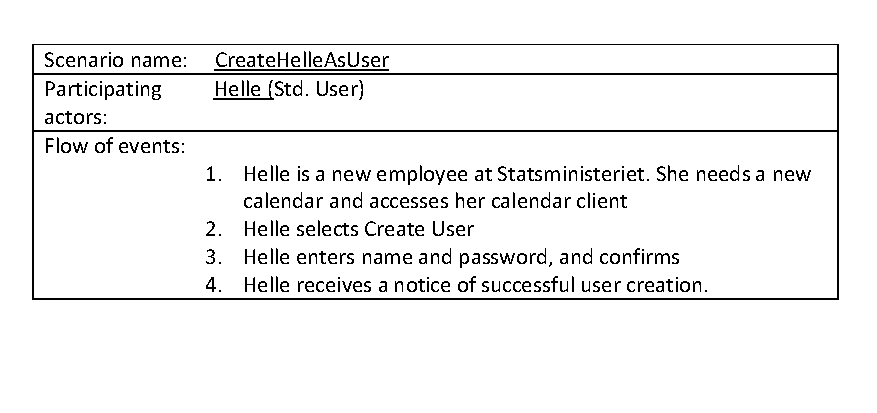
\includegraphics[scale=0.8]{docs/ScCreateUser.pdf}}
			
			Note: We need to figure out how to handle user-relationsship. 
			It is unlikely everybody able to invite all users. Do we have user-friendship, groups.. etc?

		\subsubsection{Use case model}
			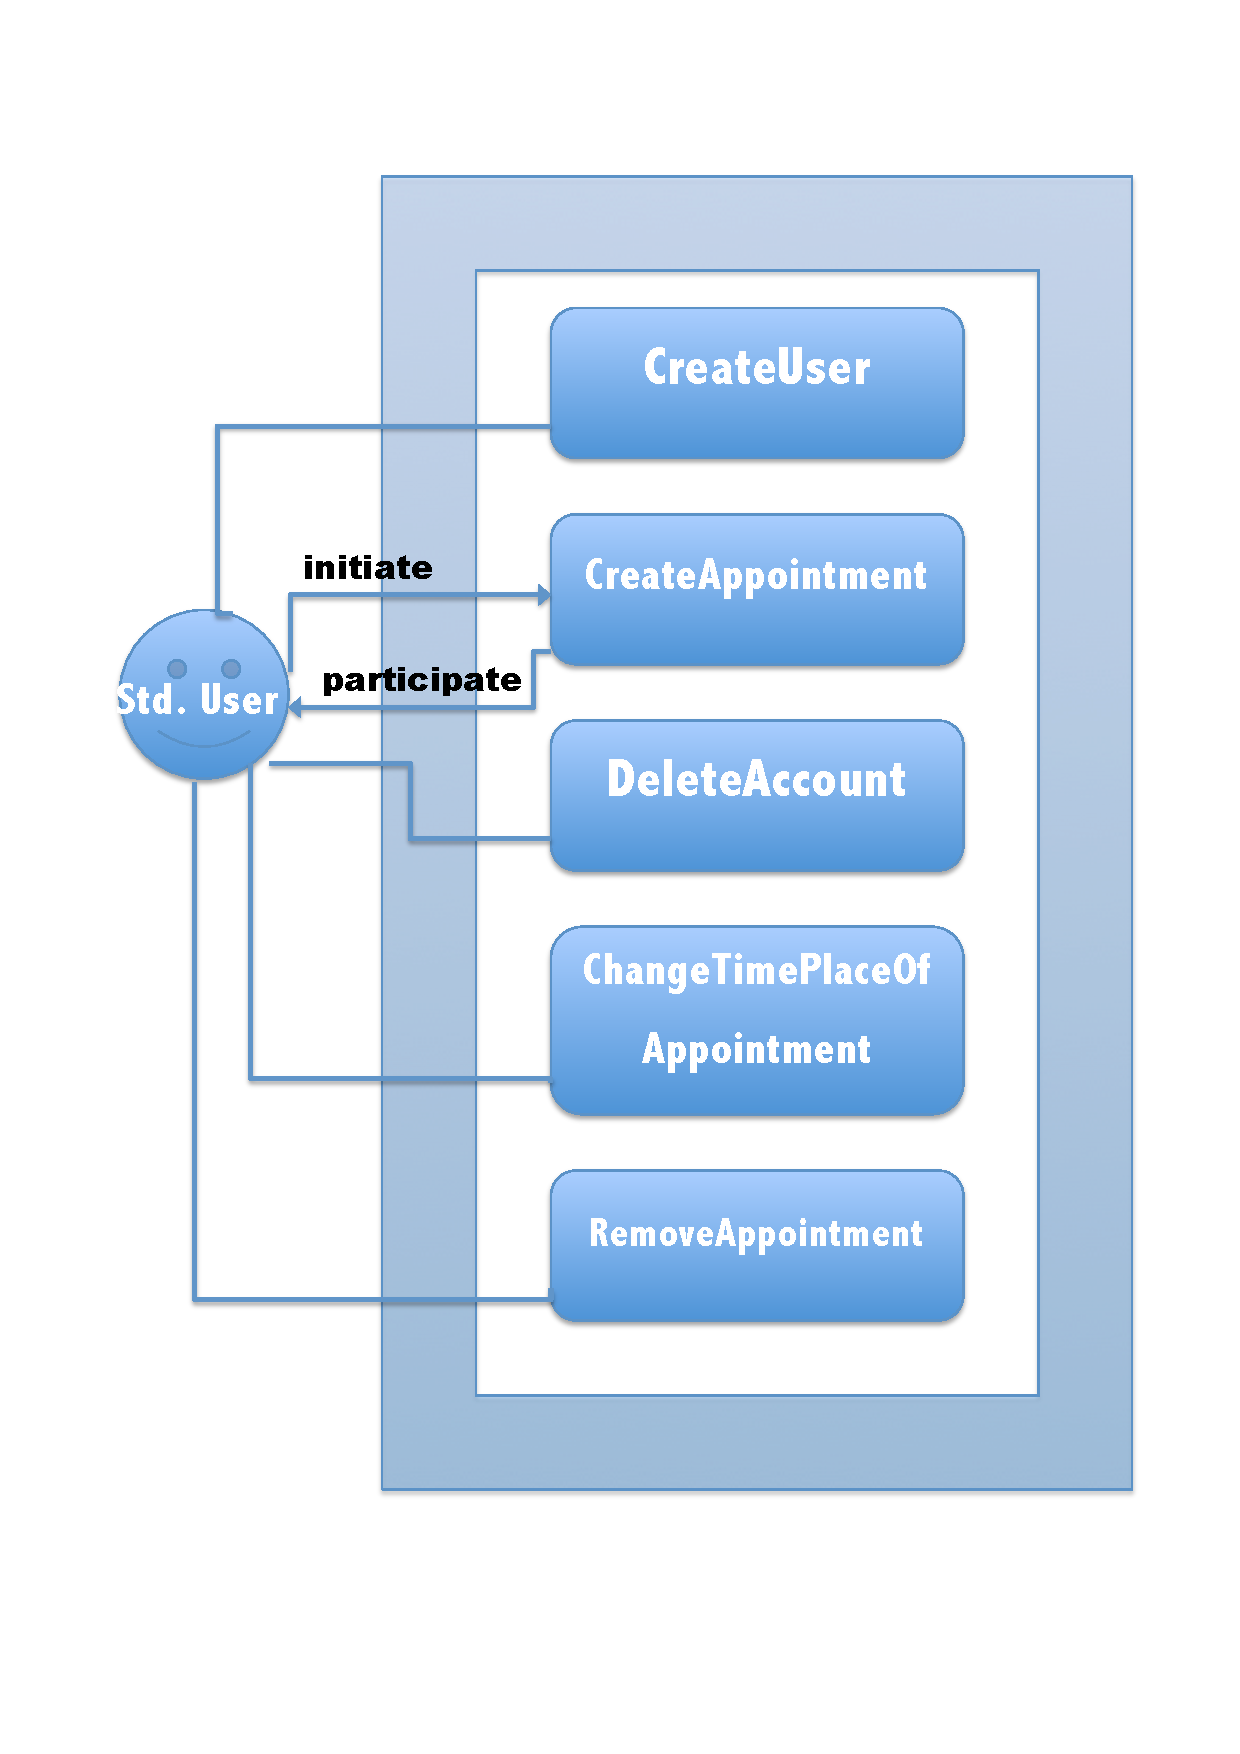
\includepdf[scale=0.7]{docs/UMLUsecaseDiagramCALENDAR.pdf}
			\begin{center}	
				{\tabulinesep=1.2mm
\begin{tabu}{ | p{3cm} | p{13cm} |}
    \hline
    Use case name: 			& 		CreateAppointment\\ \hline
    Participating  			& 		User wants to create an appointment with some friends and seeks additional participants. \\
    actors:					&		Users invited to the appointment.\\ \hline
    Flow of events: 		& 		1. User opens Calendar. \\
							&		2. Calendar shows the calendar navigation.\\
							&		3. User selects the date and time of the appointment.\\
							&		4. Calendar shows a form for entering description and place and participants.\\
							&		5. User fills the form, adds participants through email and enters how many additional participants he seeks.\\
							&		6. Calendar creates the appointment and notify participants that they have been added to the event.\\
							&		7. Her er en øndring i denne usacase.\\ \hline
    Entry condition: 		& 		- User is logged in  \\ \hline
	Exit conditions: 		&		- Appointment is changed.\\
							&		- User close the system.\\
							&		- Connection lost.\\\hline
	Quality requirements	&	 	- None \\\hline
\end{tabu}
}\\
				{\tabulinesep=1.2mm
\begin{tabu}{ | p{3cm} | p{13cm} |}
    \hline
    Use case name: 			& 		EditAppointment\\ \hline
    Participating  			& 		User wants to edit time and date of an appointment. \\
    actors:					& 		\\ \hline
    Flow of events: 		& 		1. User opens Calender. \\
							&		2. Calender shows the calender navigation.\\
							&		3. User selects the appointment he wants to change.\\
							&		4. Calender shows the appointment in normal mode that allows changes.\\
							&		5. User enters submits the wished changes.\\
							&		6. Calender updates the appointment and notify potential participants about the changes.\\ \hline
    Entry condition: 		& 		- User is logged in  \\ \hline
	Exit conditions: 		&		- Appointment is changed.\\
							&		- User close the system.\\
							&		- Connection lost.\\\hline
	Quality requirements	&	 	- None \\\hline
\end{tabu}
}\\
				{\tabulinesep=1.2mm
\begin{tabu}{ | p{3cm} | p{13cm} |}
    \hline
    Use case name: 			& 		DeleteAccount\\ \hline
    Participating  			& 		User wants to delete her account. \\
    actors:					&		Other users effected by deletion.\\ \hline
    Flow of events: 		& 		1. User opens the program. \\
							&		2. Calendar shows the calendar navigation.\\
							&		3. User selects edit profile.\\
							&		4. Calendar shows the profile edit.\\
							&		5. User select delete account.\\
							&		6. Calendar removes the user from all appointment. If the user was the only participant, the appointment is deleted.\\
							&		7. Calendar deletes account, and notifies other users about changes made to their appointments. \\\hline
    Entry condition: 		& 		- User is logged in  \\ \hline
	Exit conditions: 		&		- User account is deleted.\\
							&		- User close the system.\\
							&		- Connection lost.\\\hline
	Quality requirements	&	 	- None \\\hline
\end{tabu}
}\\
				{\tabulinesep=1.2mm
\begin{tabu}{ | p{3cm} | p{13cm} |}
    \hline
    Use case name: 			& 		DeleteAppointment\\ \hline
    Participating  			& 		User wants to delete an appointment. \\
    actors:					&		Other users effected by deletion.\\ \hline
    Flow of events: 		& 		1. User opens LuckyCalendar. \\
							&		2. LuckyCalendar shows the calendar navigation.\\
							&		3. User selects the appointment he wants to delete.\\
							&		4. LuckyCalendar shows the appointment in normal mode that allows changes.\\
							&		5. User selects delete appointment the wished changes.\\
							&		6. LuckyCalendar changes/deletes the event accordingly and notify other participants.\\\hline
    Entry condition: 		& 		- User is logged in.  \\ \hline
	Exit conditions: 		&		- Appointment is deleted.\\
							&		- User closes the system.\\
							&		- Connection lost.\\\hline
	Quality requirements	&	 	- None \\\hline
\end{tabu}
}\\
			\end{center}
		\subsubsection{Object model}
		\subsubsection{Dynamic model}
		\subsubsection{User interface}
	\newpage

\section{Subsystem services}
	Our system works primarily on the server subsystem, where the connections are handled, where the Appointments, LuckyAppointments, UserData and Notifications are retrieved from  and where the data is saved. Our two other main Subsystems; the LuckyMatchFinder and the Client, only works with their own data retrieved from the server, before again saving it on the server (or locally in case of the Client having no network connection to the server). Those two subsystems does not as such provide any services. 

Server services:
\begin{enumerate}
\item ConnectionManager - Used by the Client subsystem to get a Connection to the server.
\item AppointmentRequester - Used by the Client and LuckyMatchFinder to retrieve the relevant Appointments.
\item LuckyAppointmentRequester - Used by the Client and LuckyMatchFinder to retrieve the relevant LuckyAppointments.
\item NotificationRequester - Used by the Client to retrieve Notifications.
\item UserDataRequester - Used by the Client for retrieving data about users.
\item DataSaving -  Used by the Client and the LuckyMatchFInder for Saving all data to the server.
\end{enumerate}

	\newpage

\section{Glossary}
	\subsection{Initial Analysis Objects:}
	{\tabulinesep=1.2mm
\begin{tabu}{ | p{3cm} | p{13cm} |}\hline
    Object name 			& 		Description\\\hline
    Account 				& 		An account keeps track of user information, and may participate or create in an \uline{appointment} or a \uline{luckyAppointment}. \\\hline
	Appointment				&		A digital representation of an appointment between 1 or more \uline{Users}. It contains a time and a \uline{place} for the appointment, a title and a description for the event.\\\hline
	LuckyAppointment		&		A representation of the time space, the \uline{user} wishes to join an \uline{appointment} with another \uline{user}. It contains a desired time frame and city.\\\hline
	Reccuring-Appointment	&		An \uline{appointment} that happens several times, \uline{appointments} are created at the time of the ReccuringAppointment. Might have room for lucky participants, but a LuckyAppointment can't be a RecurringAppointment. \\ \hline
    Place 					& 		A digital representation of a space, might be none-existing. It contains a city.\\\hline
	Calendar				&		An collection of \uline{appointments} for one \uline{account}.\\ \hline
    City 					& 		A digital representation of a city, identified by the postal code.\\\hline
	LuckyParticipant		&		A user participating an event through a \uline{LuckyAppointment}.\\\hline
	Participant: 			&		How an \uline{account} (and thereby \uline{user}). Is tied to an appointment.\\\hline
    User  					& 		User a person who owns an \uline{account} and thereby a \uline{calender}. He is able to create/delete/edit \uline{appointments} and  \uline{luckyAppointments}. Must be authorized by the server, otherwise the user is a \uline{Guest} \\\hline
    Guest					&		A person who is using the system, but is not logged in (i.e. not authorized by the server). A \uline{Guest} is only able to create a new user, or log in \\\hline
    ServerAdmin				&		A person who is responsible for administrating the servers. At present his only job is to turn on/off the server in case of failure \\\hline
\end{tabu}
}
	\newpage


\end{document}

